% !TEX root=maha-dip-notes.tex
\documentclass{report}
\usepackage[tmargin=2cm,rmargin=1in,lmargin=1in,margin=0.85in,bmargin=2cm,footskip=.2in]{geometry}
\usepackage{amsmath,amsfonts,amsthm,amssymb,mathtools}
\usepackage[varbb]{newpxmath}
\usepackage{xfrac}
\usepackage[makeroom]{cancel}
\usepackage{mathtools}
\usepackage{bookmark}
\usepackage{enumitem}
\usepackage{hyperref,theoremref}
\hypersetup{
	pdftitle={Assignment},
	colorlinks=true, linkcolor=doc!90,
	bookmarksnumbered=true,
	bookmarksopen=true
}
\usepackage[most,many,breakable]{tcolorbox}
\usepackage{xcolor}
\usepackage{varwidth}
\usepackage{varwidth}
\usepackage{etoolbox}
%\usepackage{authblk}
\usepackage{nameref}
\usepackage{multicol,array}
\usepackage[ruled,vlined,linesnumbered]{algorithm2e}
\usepackage{comment} % enables the use of multi-line comments (\ifx \fi) 
\usepackage{import}
\usepackage{xifthen}
\usepackage{pdfpages}
\usepackage{transparent}


\newcommand\mycommfont[1]{\footnotesize\ttfamily\textcolor{blue}{#1}}
\SetCommentSty{mycommfont}
\newcommand{\incfig}[1]{%
    \def\svgwidth{\columnwidth}
    \import{./figures/}{#1.pdf_tex}
}

\usepackage{tikzsymbols}
\renewcommand\qedsymbol{$\Laughey$}


\usepackage{graphicx}
\usepackage{booktabs,array,multirow}
\usepackage{siunitx}
\usepackage{tikz}
\usepackage{pgfplots}
\pgfplotsset{compat=1.18}
\usetikzlibrary{arrows.meta,positioning,calc}


%\usepackage{import}
%\usepackage{xifthen}
%\usepackage{pdfpages}
%\usepackage{transparent}


%%%%%%%%%%%%%%%%%%%%%%%%%%%%%%
% SELF MADE COLORS
%%%%%%%%%%%%%%%%%%%%%%%%%%%%%%



\definecolor{myg}{RGB}{56, 140, 70}
\definecolor{myb}{RGB}{45, 111, 177}
\definecolor{myr}{RGB}{199, 68, 64}
\definecolor{mytheorembg}{HTML}{F2F2F9}
\definecolor{mytheoremfr}{HTML}{00007B}
\definecolor{mylenmabg}{HTML}{FFFAF8}
\definecolor{mylenmafr}{HTML}{983b0f}
\definecolor{mypropbg}{HTML}{f2fbfc}
\definecolor{mypropfr}{HTML}{191971}
\definecolor{myexamplebg}{HTML}{F2FBF8}
\definecolor{myexamplefr}{HTML}{88D6D1}
\definecolor{myexampleti}{HTML}{2A7F7F}
\definecolor{mydefinitbg}{HTML}{E5E5FF}
\definecolor{mydefinitfr}{HTML}{3F3FA3}
\definecolor{notesgreen}{RGB}{0,162,0}
\definecolor{myp}{RGB}{197, 92, 212}
\definecolor{mygr}{HTML}{2C3338}
\definecolor{myred}{RGB}{127,0,0}
\definecolor{myyellow}{RGB}{169,121,69}
\definecolor{myexercisebg}{HTML}{F2FBF8}
\definecolor{myexercisefg}{HTML}{88D6D1}



%%%%%%%%%%%%%%%%%%%%%%%%%%%%
% TCOLORBOX SETUPS
%%%%%%%%%%%%%%%%%%%%%%%%%%%%

\setlength{\parindent}{1cm}
%================================
% THEOREM BOX
%================================

\tcbuselibrary{theorems,skins,hooks}
\newtcbtheorem[number within=section]{Theorem}{Theorem}
{%
	enhanced,
	breakable,
	colback = mytheorembg,
	frame hidden,
	boxrule = 0sp,
	borderline west = {2pt}{0pt}{mytheoremfr},
	sharp corners,
	detach title,
	before upper = \tcbtitle\par\smallskip,
	coltitle = mytheoremfr,
	fonttitle = \bfseries\sffamily,
	description font = \mdseries,
	separator sign none,
	segmentation style={solid, mytheoremfr},
}
{th}

\tcbuselibrary{theorems,skins,hooks}
\newtcbtheorem[number within=chapter]{theorem}{Theorem}
{%
	enhanced,
	breakable,
	colback = mytheorembg,
	frame hidden,
	boxrule = 0sp,
	borderline west = {2pt}{0pt}{mytheoremfr},
	sharp corners,
	detach title,
	before upper = \tcbtitle\par\smallskip,
	coltitle = mytheoremfr,
	fonttitle = \bfseries\sffamily,
	description font = \mdseries,
	separator sign none,
	segmentation style={solid, mytheoremfr},
}
{th}


\tcbuselibrary{theorems,skins,hooks}
\newtcolorbox{Theoremcon}
{%
	enhanced
	,breakable
	,colback = mytheorembg
	,frame hidden
	,boxrule = 0sp
	,borderline west = {2pt}{0pt}{mytheoremfr}
	,sharp corners
	,description font = \mdseries
	,separator sign none
}

%================================
% Corollery
%================================
\tcbuselibrary{theorems,skins,hooks}
\newtcbtheorem[number within=section]{Corollary}{Corollary}
{%
	enhanced
	,breakable
	,colback = myp!10
	,frame hidden
	,boxrule = 0sp
	,borderline west = {2pt}{0pt}{myp!85!black}
	,sharp corners
	,detach title
	,before upper = \tcbtitle\par\smallskip
	,coltitle = myp!85!black
	,fonttitle = \bfseries\sffamily
	,description font = \mdseries
	,separator sign none
	,segmentation style={solid, myp!85!black}
}
{th}
\tcbuselibrary{theorems,skins,hooks}
\newtcbtheorem[number within=chapter]{corollary}{Corollary}
{%
	enhanced
	,breakable
	,colback = myp!10
	,frame hidden
	,boxrule = 0sp
	,borderline west = {2pt}{0pt}{myp!85!black}
	,sharp corners
	,detach title
	,before upper = \tcbtitle\par\smallskip
	,coltitle = myp!85!black
	,fonttitle = \bfseries\sffamily
	,description font = \mdseries
	,separator sign none
	,segmentation style={solid, myp!85!black}
}
{th}


%================================
% LEMMA
%================================

\tcbuselibrary{theorems,skins,hooks}
\newtcbtheorem[number within=section]{Lemma}{Lemma}
{%
	enhanced,
	breakable,
	colback = mylenmabg,
	frame hidden,
	boxrule = 0sp,
	borderline west = {2pt}{0pt}{mylenmafr},
	sharp corners,
	detach title,
	before upper = \tcbtitle\par\smallskip,
	coltitle = mylenmafr,
	fonttitle = \bfseries\sffamily,
	description font = \mdseries,
	separator sign none,
	segmentation style={solid, mylenmafr},
}
{th}

\tcbuselibrary{theorems,skins,hooks}
\newtcbtheorem[number within=chapter]{lenma}{Lenma}
{%
	enhanced,
	breakable,
	colback = mylenmabg,
	frame hidden,
	boxrule = 0sp,
	borderline west = {2pt}{0pt}{mylenmafr},
	sharp corners,
	detach title,
	before upper = \tcbtitle\par\smallskip,
	coltitle = mylenmafr,
	fonttitle = \bfseries\sffamily,
	description font = \mdseries,
	separator sign none,
	segmentation style={solid, mylenmafr},
}
{th}

%================================
% Exercise
%================================

\tcbuselibrary{theorems,skins,hooks}
\newtcbtheorem[number within=section]{Exercise}{Exercise}
{%
	enhanced,
	breakable,
	colback = myexercisebg,
	frame hidden,
	boxrule = 0sp,
	borderline west = {2pt}{0pt}{myexercisefg},
	sharp corners,
	detach title,
	before upper = \tcbtitle\par\smallskip,
	coltitle = myexercisefg,
	fonttitle = \bfseries\sffamily,
	description font = \mdseries,
	separator sign none,
	segmentation style={solid, myexercisefg},
}
{th}

\tcbuselibrary{theorems,skins,hooks}
\newtcbtheorem[number within=chapter]{exercise}{Exercise}
{%
	enhanced,
	breakable,
	colback = myexercisebg,
	frame hidden,
	boxrule = 0sp,
	borderline west = {2pt}{0pt}{myexercisefg},
	sharp corners,
	detach title,
	before upper = \tcbtitle\par\smallskip,
	coltitle = myexercisefg,
	fonttitle = \bfseries\sffamily,
	description font = \mdseries,
	separator sign none,
	segmentation style={solid, myexercisefg},
}
{th}



%================================
% PROPOSITION
%================================

\tcbuselibrary{theorems,skins,hooks}
\newtcbtheorem[number within=section]{Prop}{Proposition}
{%
	enhanced,
	breakable,
	colback = mypropbg,
	frame hidden,
	boxrule = 0sp,
	borderline west = {2pt}{0pt}{mypropfr},
	sharp corners,
	detach title,
	before upper = \tcbtitle\par\smallskip,
	coltitle = mypropfr,
	fonttitle = \bfseries\sffamily,
	description font = \mdseries,
	separator sign none,
	segmentation style={solid, mypropfr},
}
{th}

\tcbuselibrary{theorems,skins,hooks}
\newtcbtheorem[number within=chapter]{prop}{Proposition}
{%
	enhanced,
	breakable,
	colback = mypropbg,
	frame hidden,
	boxrule = 0sp,
	borderline west = {2pt}{0pt}{mypropfr},
	sharp corners,
	detach title,
	before upper = \tcbtitle\par\smallskip,
	coltitle = mypropfr,
	fonttitle = \bfseries\sffamily,
	description font = \mdseries,
	separator sign none,
	segmentation style={solid, mypropfr},
}
{th}


%================================
% CLAIM
%================================

\tcbuselibrary{theorems,skins,hooks}
\newtcbtheorem[number within=section]{claim}{Claim}
{%
	enhanced
	,breakable
	,colback = myg!10
	,frame hidden
	,boxrule = 0sp
	,borderline west = {2pt}{0pt}{myg}
	,sharp corners
	,detach title
	,before upper = \tcbtitle\par\smallskip
	,coltitle = myg!85!black
	,fonttitle = \bfseries\sffamily
	,description font = \mdseries
	,separator sign none
	,segmentation style={solid, myg!85!black}
}
{th}




%================================
% EXAMPLE BOX
%================================

\newtcbtheorem[number within=section]{Example}{Example}
{%
	colback = myexamplebg
	,breakable
	,colframe = myexamplefr
	,coltitle = myexampleti
	,boxrule = 1pt
	,sharp corners
	,detach title
	,before upper=\tcbtitle\par\smallskip
	,fonttitle = \bfseries
	,description font = \mdseries
	,separator sign none
	,description delimiters parenthesis
}
{ex}

\newtcbtheorem[number within=chapter]{example}{Example}
{%
	colback = myexamplebg
	,breakable
	,colframe = myexamplefr
	,coltitle = myexampleti
	,boxrule = 1pt
	,sharp corners
	,detach title
	,before upper=\tcbtitle\par\smallskip
	,fonttitle = \bfseries
	,description font = \mdseries
	,separator sign none
	,description delimiters parenthesis
}
{ex}

%================================
% DEFINITION BOX
%================================

\newtcbtheorem[number within=section]{Definition}{Definition}{enhanced,
	before skip=2mm,after skip=2mm, colback=red!5,colframe=red!80!black,boxrule=0.5mm,
	attach boxed title to top left={xshift=1cm,yshift*=1mm-\tcboxedtitleheight}, varwidth boxed title*=-3cm,
	boxed title style={frame code={
					\path[fill=tcbcolback]
					([yshift=-1mm,xshift=-1mm]frame.north west)
					arc[start angle=0,end angle=180,radius=1mm]
					([yshift=-1mm,xshift=1mm]frame.north east)
					arc[start angle=180,end angle=0,radius=1mm];
					\path[left color=tcbcolback!60!black,right color=tcbcolback!60!black,
						middle color=tcbcolback!80!black]
					([xshift=-2mm]frame.north west) -- ([xshift=2mm]frame.north east)
					[rounded corners=1mm]-- ([xshift=1mm,yshift=-1mm]frame.north east)
					-- (frame.south east) -- (frame.south west)
					-- ([xshift=-1mm,yshift=-1mm]frame.north west)
					[sharp corners]-- cycle;
				},interior engine=empty,
		},
	fonttitle=\bfseries,
	title={#2},#1}{def}
\newtcbtheorem[number within=chapter]{definition}{Definition}{enhanced,
	before skip=2mm,after skip=2mm, colback=red!5,colframe=red!80!black,boxrule=0.5mm,
	attach boxed title to top left={xshift=1cm,yshift*=1mm-\tcboxedtitleheight}, varwidth boxed title*=-3cm,
	boxed title style={frame code={
					\path[fill=tcbcolback]
					([yshift=-1mm,xshift=-1mm]frame.north west)
					arc[start angle=0,end angle=180,radius=1mm]
					([yshift=-1mm,xshift=1mm]frame.north east)
					arc[start angle=180,end angle=0,radius=1mm];
					\path[left color=tcbcolback!60!black,right color=tcbcolback!60!black,
						middle color=tcbcolback!80!black]
					([xshift=-2mm]frame.north west) -- ([xshift=2mm]frame.north east)
					[rounded corners=1mm]-- ([xshift=1mm,yshift=-1mm]frame.north east)
					-- (frame.south east) -- (frame.south west)
					-- ([xshift=-1mm,yshift=-1mm]frame.north west)
					[sharp corners]-- cycle;
				},interior engine=empty,
		},
	fonttitle=\bfseries,
	title={#2},#1}{def}



%================================
% EXERCISE BOX
%================================

\makeatletter
\newtcbtheorem{question}{Question}{enhanced,
	breakable,
	colback=white,
	colframe=myb!80!black,
	attach boxed title to top left={yshift*=-\tcboxedtitleheight},
	fonttitle=\bfseries,
	title={#2},
	boxed title size=title,
	boxed title style={%
			sharp corners,
			rounded corners=northwest,
			colback=tcbcolframe,
			boxrule=0pt,
		},
	underlay boxed title={%
			\path[fill=tcbcolframe] (title.south west)--(title.south east)
			to[out=0, in=180] ([xshift=5mm]title.east)--
			(title.center-|frame.east)
			[rounded corners=\kvtcb@arc] |-
			(frame.north) -| cycle;
		},
	#1
}{def}
\makeatother

%================================
% SOLUTION BOX
%================================

\makeatletter
\newtcolorbox{solution}{enhanced,
	breakable,
	colback=white,
	colframe=myg!80!black,
	attach boxed title to top left={yshift*=-\tcboxedtitleheight},
	title=Solution,
	boxed title size=title,
	boxed title style={%
			sharp corners,
			rounded corners=northwest,
			colback=tcbcolframe,
			boxrule=0pt,
		},
	underlay boxed title={%
			\path[fill=tcbcolframe] (title.south west)--(title.south east)
			to[out=0, in=180] ([xshift=5mm]title.east)--
			(title.center-|frame.east)
			[rounded corners=\kvtcb@arc] |-
			(frame.north) -| cycle;
		},
}
\makeatother

%================================
% Question BOX
%================================

\makeatletter
\newtcbtheorem{qstion}{Question}{enhanced,
	breakable,
	colback=white,
	colframe=mygr,
	attach boxed title to top left={yshift*=-\tcboxedtitleheight},
	fonttitle=\bfseries,
	title={#2},
	boxed title size=title,
	boxed title style={%
			sharp corners,
			rounded corners=northwest,
			colback=tcbcolframe,
			boxrule=0pt,
		},
	underlay boxed title={%
			\path[fill=tcbcolframe] (title.south west)--(title.south east)
			to[out=0, in=180] ([xshift=5mm]title.east)--
			(title.center-|frame.east)
			[rounded corners=\kvtcb@arc] |-
			(frame.north) -| cycle;
		},
	#1
}{def}
\makeatother

\newtcbtheorem[number within=chapter]{wconc}{Wrong Concept}{
	breakable,
	enhanced,
	colback=white,
	colframe=myr,
	arc=0pt,
	outer arc=0pt,
	fonttitle=\bfseries\sffamily\large,
	colbacktitle=myr,
	attach boxed title to top left={},
	boxed title style={
			enhanced,
			skin=enhancedfirst jigsaw,
			arc=3pt,
			bottom=0pt,
			interior style={fill=myr}
		},
	#1
}{def}



%================================
% NOTE BOX
%================================

\usetikzlibrary{arrows,calc,shadows.blur}
\tcbuselibrary{skins}
\newtcolorbox{note}[1][]{%
	enhanced jigsaw,
	colback=gray!20!white,%
	colframe=gray!80!black,
	size=small,
	boxrule=1pt,
	title=\textbf{Note:-},
	halign title=flush center,
	coltitle=black,
	breakable,
	drop shadow=black!50!white,
	attach boxed title to top left={xshift=1cm,yshift=-\tcboxedtitleheight/2,yshifttext=-\tcboxedtitleheight/2},
	minipage boxed title=1.5cm,
	boxed title style={%
			colback=white,
			size=fbox,
			boxrule=1pt,
			boxsep=2pt,
			underlay={%
					\coordinate (dotA) at ($(interior.west) + (-0.5pt,0)$);
					\coordinate (dotB) at ($(interior.east) + (0.5pt,0)$);
					\begin{scope}
						\clip (interior.north west) rectangle ([xshift=3ex]interior.east);
						\filldraw [white, blur shadow={shadow opacity=60, shadow yshift=-.75ex}, rounded corners=2pt] (interior.north west) rectangle (interior.south east);
					\end{scope}
					\begin{scope}[gray!80!black]
						\fill (dotA) circle (2pt);
						\fill (dotB) circle (2pt);
					\end{scope}
				},
		},
	#1,
}

%%%%%%%%%%%%%%%%%%%%%%%%%%%%%%
% SELF MADE COMMANDS
%%%%%%%%%%%%%%%%%%%%%%%%%%%%%%


\newcommand{\thm}[2]{\begin{Theorem}{#1}{}#2\end{Theorem}}
\newcommand{\cor}[2]{\begin{Corollary}{#1}{}#2\end{Corollary}}
\newcommand{\mlenma}[2]{\begin{Lemma}{#1}{}#2\end{Lemma}}
\newcommand{\mer}[2]{\begin{Exercise}{#1}{}#2\end{Exercise}}
\newcommand{\mprop}[2]{\begin{Prop}{#1}{}#2\end{Prop}}
\newcommand{\clm}[3]{\begin{claim}{#1}{#2}#3\end{claim}}
\newcommand{\wc}[2]{\begin{wconc}{#1}{}\setlength{\parindent}{1cm}#2\end{wconc}}
\newcommand{\thmcon}[1]{\begin{Theoremcon}{#1}\end{Theoremcon}}
\newcommand{\ex}[2]{\begin{Example}{#1}{}#2\end{Example}}
\newcommand{\dfn}[2]{\begin{Definition}[colbacktitle=red!75!black]{#1}{}#2\end{Definition}}
\newcommand{\dfnc}[2]{\begin{definition}[colbacktitle=red!75!black]{#1}{}#2\end{definition}}
\newcommand{\qs}[2]{\begin{question}{#1}{}#2\end{question}}
\newcommand{\pf}[2]{\begin{myproof}[#1]#2\end{myproof}}
\newcommand{\nt}[1]{\begin{note}#1\end{note}}

\newcommand*\circled[1]{\tikz[baseline=(char.base)]{
		\node[shape=circle,draw,inner sep=1pt] (char) {#1};}}
\newcommand\getcurrentref[1]{%
	\ifnumequal{\value{#1}}{0}
	{??}
	{\the\value{#1}}%
}
\newcommand{\getCurrentSectionNumber}{\getcurrentref{section}}
\newenvironment{myproof}[1][\proofname]{%
	\proof[\bfseries #1: ]%
}{\endproof}

\newcommand{\mclm}[2]{\begin{myclaim}[#1]#2\end{myclaim}}
\newenvironment{myclaim}[1][\claimname]{\proof[\bfseries #1: ]}{}
\newenvironment{iclaim}[1][\claimname]{\bfseries #1\mdseries:}{}
\newcommand{\iclm}[2]{\begin{iclaim}[#1]#2\end{iclaim}}

\newcounter{mylabelcounter}

\makeatletter
\newcommand{\setword}[2]{%
	\phantomsection
	#1\def\@currentlabel{\unexpanded{#1}}\label{#2}%
}
\makeatother




\tikzset{
	symbol/.style={
			draw=none,
			every to/.append style={
					edge node={node [sloped, allow upside down, auto=false]{$#1$}}}
		}
}


% deliminators
\DeclarePairedDelimiter{\abs}{\lvert}{\rvert}
\DeclarePairedDelimiter{\norm}{\lVert}{\rVert}

\DeclarePairedDelimiter{\ceil}{\lceil}{\rceil}
\DeclarePairedDelimiter{\floor}{\lfloor}{\rfloor}
\DeclarePairedDelimiter{\round}{\lfloor}{\rceil}

\newsavebox\diffdbox
\newcommand{\slantedromand}{{\mathpalette\makesl{d}}}
\newcommand{\makesl}[2]{%
\begingroup
\sbox{\diffdbox}{$\mathsurround=0pt#1\mathrm{#2}$}%
\pdfsave
\pdfsetmatrix{1 0 0.2 1}%
\rlap{\usebox{\diffdbox}}%
\pdfrestore
\hskip\wd\diffdbox
\endgroup
}
\newcommand{\dd}[1][]{\ensuremath{\mathop{}\!\ifstrempty{#1}{%
\slantedromand\@ifnextchar^{\hspace{0.2ex}}{\hspace{0.1ex}}}%
{\slantedromand\hspace{0.2ex}^{#1}}}}
\ProvideDocumentCommand\dv{o m g}{%
  \ensuremath{%
    \IfValueTF{#3}{%
      \IfNoValueTF{#1}{%
        \frac{\dd #2}{\dd #3}%
      }{%
        \frac{\dd^{#1} #2}{\dd #3^{#1}}%
      }%
    }{%
      \IfNoValueTF{#1}{%
        \frac{\dd}{\dd #2}%
      }{%
        \frac{\dd^{#1}}{\dd #2^{#1}}%
      }%
    }%
  }%
}
\providecommand*{\pdv}[3][]{\frac{\partial^{#1}#2}{\partial#3^{#1}}}
%  - others
\DeclareMathOperator{\Lap}{\mathcal{L}}
\DeclareMathOperator{\Var}{Var} % varience
\DeclareMathOperator{\Cov}{Cov} % covarience
\DeclareMathOperator{\E}{E} % expected

% Since the amsthm package isn't loaded

% I prefer the slanted \leq
\let\oldleq\leq % save them in case they're every wanted
\let\oldgeq\geq
\renewcommand{\leq}{\leqslant}
\renewcommand{\geq}{\geqslant}

% % redefine matrix env to allow for alignment, use r as default
% \renewcommand*\env@matrix[1][r]{\hskip -\arraycolsep
%     \let\@ifnextchar\new@ifnextchar
%     \array{*\c@MaxMatrixCols #1}}


%\usepackage{framed}
%\usepackage{titletoc}
%\usepackage{etoolbox}
%\usepackage{lmodern}


%\patchcmd{\tableofcontents}{\contentsname}{\sffamily\contentsname}{}{}

%\renewenvironment{leftbar}
%{\def\FrameCommand{\hspace{6em}%
%		{\color{myyellow}\vrule width 2pt depth 6pt}\hspace{1em}}%
%	\MakeFramed{\parshape 1 0cm \dimexpr\textwidth-6em\relax\FrameRestore}\vskip2pt%
%}
%{\endMakeFramed}

%\titlecontents{chapter}
%[0em]{\vspace*{2\baselineskip}}
%{\parbox{4.5em}{%
%		\hfill\Huge\sffamily\bfseries\color{myred}\thecontentspage}%
%	\vspace*{-2.3\baselineskip}\leftbar\textsc{\small\chaptername~\thecontentslabel}\\\sffamily}
%{}{\endleftbar}
%\titlecontents{section}
%[8.4em]
%{\sffamily\contentslabel{3em}}{}{}
%{\hspace{0.5em}\nobreak\itshape\color{myred}\contentspage}
%\titlecontents{subsection}
%[8.4em]
%{\sffamily\contentslabel{3em}}{}{}  
%{\hspace{0.5em}\nobreak\itshape\color{myred}\contentspage}



%%%%%%%%%%%%%%%%%%%%%%%%%%%%%%%%%%%%%%%%%%%
% TABLE OF CONTENTS
%%%%%%%%%%%%%%%%%%%%%%%%%%%%%%%%%%%%%%%%%%%

\usepackage{tikz}
\definecolor{doc}{RGB}{0,60,110}
\usepackage{titletoc}
\contentsmargin{0cm}
\titlecontents{chapter}[3.7pc]
{\addvspace{30pt}%
	\begin{tikzpicture}[remember picture, overlay]%
		\draw[fill=doc!60,draw=doc!60] (-7,-.1) rectangle (-0.9,.5);%
		\pgftext[left,x=-3.7cm,y=0.2cm]{\color{white}\Large\sc\bfseries Chapter\ \thecontentslabel};%
	\end{tikzpicture}\color{doc!60}\large\sc\bfseries}%
{}
{}
{\;\titlerule\;\large\sc\bfseries Page \thecontentspage
	\begin{tikzpicture}[remember picture, overlay]
		\draw[fill=doc!60,draw=doc!60] (2pt,0) rectangle (4,0.1pt);
	\end{tikzpicture}}%
\titlecontents{section}[3.7pc]
{\addvspace{2pt}}
{\contentslabel[\thecontentslabel]{2pc}}
{}
{\hfill\small \thecontentspage}
[]
\titlecontents*{subsection}[3.7pc]
{\addvspace{-1pt}\small}
{}
{}
{\ --- \small\thecontentspage}
[ \textbullet\ ][]

\makeatletter
\renewcommand{\tableofcontents}{%
	\chapter*{%
	  \vspace*{-20\p@}%
	  \begin{tikzpicture}[remember picture, overlay]%
		  \pgftext[right,x=15cm,y=0.2cm]{\color{doc!60}\Huge\sc\bfseries \contentsname};%
		  \draw[fill=doc!60,draw=doc!60] (13,-.75) rectangle (20,1);%
		  \clip (13,-.75) rectangle (20,1);
		  \pgftext[right,x=15cm,y=0.2cm]{\color{white}\Huge\sc\bfseries \contentsname};%
	  \end{tikzpicture}}%
	\@starttoc{toc}}
\makeatother

\newcommand{\eps}{\epsilon}
\newcommand{\veps}{\varepsilon}
\newcommand{\Qed}{\begin{flushright}\qed\end{flushright}}

\newcommand{\parinn}{\setlength{\parindent}{1cm}}
\newcommand{\parinf}{\setlength{\parindent}{0cm}}

% \newcommand{\norm}{\|\cdot\|}
\newcommand{\inorm}{\norm_{\infty}}
\newcommand{\opensets}{\{V_{\alpha}\}_{\alpha\in I}}
\newcommand{\oset}{V_{\alpha}}
\newcommand{\opset}[1]{V_{\alpha_{#1}}}
\newcommand{\lub}{\text{lub}}
\newcommand{\del}[2]{\frac{\partial #1}{\partial #2}}
\newcommand{\Del}[3]{\frac{\partial^{#1} #2}{\partial^{#1} #3}}
\newcommand{\deld}[2]{\dfrac{\partial #1}{\partial #2}}
\newcommand{\Deld}[3]{\dfrac{\partial^{#1} #2}{\partial^{#1} #3}}
\newcommand{\der}[2]{\frac{\mathrm{d} #1}{\mathrm{d} #2}}
% \newcommand{\ddd}[3]{\frac{\mathrm{d}^{#3} #1}{\mathrm{d}^{#3} #2}}
\newcommand{\lm}{\lambda}
\newcommand{\uin}{\mathbin{\rotatebox[origin=c]{90}{$\in$}}}
\newcommand{\usubset}{\mathbin{\rotatebox[origin=c]{90}{$\subset$}}}
\newcommand{\lt}{\left}
\newcommand{\rt}{\right}
\newcommand{\bs}[1]{\boldsymbol{#1}}
\newcommand{\exs}{\exists}
\newcommand{\st}{\strut}
\newcommand{\dps}[1]{\displaystyle{#1}}
\newcommand{\id}{\text{id}}


\newcommand{\sol}{\setlength{\parindent}{0cm}\textbf{\textit{Solution:}}\setlength{\parindent}{1cm} }
\newcommand{\solve}[1]{\setlength{\parindent}{0cm}\textbf{\textit{Solution: }}\setlength{\parindent}{1cm}#1 \Qed}

% number sets
\newcommand{\RR}[1][]{\ensuremath{\ifstrempty{#1}{\mathbb{R}}{\mathbb{R}^{#1}}}}
\newcommand{\NN}[1][]{\ensuremath{\ifstrempty{#1}{\mathbb{N}}{\mathbb{N}^{#1}}}}
\newcommand{\ZZ}[1][]{\ensuremath{\ifstrempty{#1}{\mathbb{Z}}{\mathbb{Z}^{#1}}}}
\newcommand{\QQ}[1][]{\ensuremath{\ifstrempty{#1}{\mathbb{Q}}{\mathbb{Q}^{#1}}}}
\newcommand{\CC}[1][]{\ensuremath{\ifstrempty{#1}{\mathbb{C}}{\mathbb{C}^{#1}}}}
\newcommand{\PP}[1][]{\ensuremath{\ifstrempty{#1}{\mathbb{P}}{\mathbb{P}^{#1}}}}
\newcommand{\HH}[1][]{\ensuremath{\ifstrempty{#1}{\mathbb{H}}{\mathbb{H}^{#1}}}}
\newcommand{\FF}[1][]{\ensuremath{\ifstrempty{#1}{\mathbb{F}}{\mathbb{F}^{#1}}}}
% expected value
\newcommand{\EE}{\ensuremath{\mathbb{E}}}

%---------------------------------------
% BlackBoard Math Fonts :-
%---------------------------------------

%Captital Letters
\newcommand{\bbA}{\mathbb{A}}	\newcommand{\bbB}{\mathbb{B}}
\newcommand{\bbC}{\mathbb{C}}	\newcommand{\bbD}{\mathbb{D}}
\newcommand{\bbE}{\mathbb{E}}	\newcommand{\bbF}{\mathbb{F}}
\newcommand{\bbG}{\mathbb{G}}	\newcommand{\bbH}{\mathbb{H}}
\newcommand{\bbI}{\mathbb{I}}	\newcommand{\bbJ}{\mathbb{J}}
\newcommand{\bbK}{\mathbb{K}}	\newcommand{\bbL}{\mathbb{L}}
\newcommand{\bbM}{\mathbb{M}}	\newcommand{\bbN}{\mathbb{N}}
\newcommand{\bbO}{\mathbb{O}}	\newcommand{\bbP}{\mathbb{P}}
\newcommand{\bbQ}{\mathbb{Q}}	\newcommand{\bbR}{\mathbb{R}}
\newcommand{\bbS}{\mathbb{S}}	\newcommand{\bbT}{\mathbb{T}}
\newcommand{\bbU}{\mathbb{U}}	\newcommand{\bbV}{\mathbb{V}}
\newcommand{\bbW}{\mathbb{W}}	\newcommand{\bbX}{\mathbb{X}}
\newcommand{\bbY}{\mathbb{Y}}	\newcommand{\bbZ}{\mathbb{Z}}

%---------------------------------------
% MathCal Fonts :-
%---------------------------------------

%Captital Letters
\newcommand{\mcA}{\mathcal{A}}	\newcommand{\mcB}{\mathcal{B}}
\newcommand{\mcC}{\mathcal{C}}	\newcommand{\mcD}{\mathcal{D}}
\newcommand{\mcE}{\mathcal{E}}	\newcommand{\mcF}{\mathcal{F}}
\newcommand{\mcG}{\mathcal{G}}	\newcommand{\mcH}{\mathcal{H}}
\newcommand{\mcI}{\mathcal{I}}	\newcommand{\mcJ}{\mathcal{J}}
\newcommand{\mcK}{\mathcal{K}}	\newcommand{\mcL}{\mathcal{L}}
\newcommand{\mcM}{\mathcal{M}}	\newcommand{\mcN}{\mathcal{N}}
\newcommand{\mcO}{\mathcal{O}}	\newcommand{\mcP}{\mathcal{P}}
\newcommand{\mcQ}{\mathcal{Q}}	\newcommand{\mcR}{\mathcal{R}}
\newcommand{\mcS}{\mathcal{S}}	\newcommand{\mcT}{\mathcal{T}}
\newcommand{\mcU}{\mathcal{U}}	\newcommand{\mcV}{\mathcal{V}}
\newcommand{\mcW}{\mathcal{W}}	\newcommand{\mcX}{\mathcal{X}}
\newcommand{\mcY}{\mathcal{Y}}	\newcommand{\mcZ}{\mathcal{Z}}



%---------------------------------------
% Bold Math Fonts :-
%---------------------------------------

%Captital Letters
\newcommand{\bmA}{\boldsymbol{A}}	\newcommand{\bmB}{\boldsymbol{B}}
\newcommand{\bmC}{\boldsymbol{C}}	\newcommand{\bmD}{\boldsymbol{D}}
\newcommand{\bmE}{\boldsymbol{E}}	\newcommand{\bmF}{\boldsymbol{F}}
\newcommand{\bmG}{\boldsymbol{G}}	\newcommand{\bmH}{\boldsymbol{H}}
\newcommand{\bmI}{\boldsymbol{I}}	\newcommand{\bmJ}{\boldsymbol{J}}
\newcommand{\bmK}{\boldsymbol{K}}	\newcommand{\bmL}{\boldsymbol{L}}
\newcommand{\bmM}{\boldsymbol{M}}	\newcommand{\bmN}{\boldsymbol{N}}
\newcommand{\bmO}{\boldsymbol{O}}	\newcommand{\bmP}{\boldsymbol{P}}
\newcommand{\bmQ}{\boldsymbol{Q}}	\newcommand{\bmR}{\boldsymbol{R}}
\newcommand{\bmS}{\boldsymbol{S}}	\newcommand{\bmT}{\boldsymbol{T}}
\newcommand{\bmU}{\boldsymbol{U}}	\newcommand{\bmV}{\boldsymbol{V}}
\newcommand{\bmW}{\boldsymbol{W}}	\newcommand{\bmX}{\boldsymbol{X}}
\newcommand{\bmY}{\boldsymbol{Y}}	\newcommand{\bmZ}{\boldsymbol{Z}}
%Small Letters
\newcommand{\bma}{\boldsymbol{a}}	\newcommand{\bmb}{\boldsymbol{b}}
\newcommand{\bmc}{\boldsymbol{c}}	\newcommand{\bmd}{\boldsymbol{d}}
\newcommand{\bme}{\boldsymbol{e}}	\newcommand{\bmf}{\boldsymbol{f}}
\newcommand{\bmg}{\boldsymbol{g}}	\newcommand{\bmh}{\boldsymbol{h}}
\newcommand{\bmi}{\boldsymbol{i}}	\newcommand{\bmj}{\boldsymbol{j}}
\newcommand{\bmk}{\boldsymbol{k}}	\newcommand{\bml}{\boldsymbol{l}}
\newcommand{\bmm}{\boldsymbol{m}}	\newcommand{\bmn}{\boldsymbol{n}}
\newcommand{\bmo}{\boldsymbol{o}}	\newcommand{\bmp}{\boldsymbol{p}}
\newcommand{\bmq}{\boldsymbol{q}}	\newcommand{\bmr}{\boldsymbol{r}}
\newcommand{\bms}{\boldsymbol{s}}	\newcommand{\bmt}{\boldsymbol{t}}
\newcommand{\bmu}{\boldsymbol{u}}	\newcommand{\bmv}{\boldsymbol{v}}
\newcommand{\bmw}{\boldsymbol{w}}	\newcommand{\bmx}{\boldsymbol{x}}
\newcommand{\bmy}{\boldsymbol{y}}	\newcommand{\bmz}{\boldsymbol{z}}

%---------------------------------------
% Scr Math Fonts :-
%---------------------------------------

\newcommand{\sA}{{\mathscr{A}}}   \newcommand{\sB}{{\mathscr{B}}}
\newcommand{\sC}{{\mathscr{C}}}   \newcommand{\sD}{{\mathscr{D}}}
\newcommand{\sE}{{\mathscr{E}}}   \newcommand{\sF}{{\mathscr{F}}}
\newcommand{\sG}{{\mathscr{G}}}   \newcommand{\sH}{{\mathscr{H}}}
\newcommand{\sI}{{\mathscr{I}}}   \newcommand{\sJ}{{\mathscr{J}}}
\newcommand{\sK}{{\mathscr{K}}}   \newcommand{\sL}{{\mathscr{L}}}
\newcommand{\sM}{{\mathscr{M}}}   \newcommand{\sN}{{\mathscr{N}}}
\newcommand{\sO}{{\mathscr{O}}}   \newcommand{\sP}{{\mathscr{P}}}
\newcommand{\sQ}{{\mathscr{Q}}}   \newcommand{\sR}{{\mathscr{R}}}
\newcommand{\sS}{{\mathscr{S}}}   \newcommand{\sT}{{\mathscr{T}}}
\newcommand{\sU}{{\mathscr{U}}}   \newcommand{\sV}{{\mathscr{V}}}
\newcommand{\sW}{{\mathscr{W}}}   \newcommand{\sX}{{\mathscr{X}}}
\newcommand{\sY}{{\mathscr{Y}}}   \newcommand{\sZ}{{\mathscr{Z}}}


%---------------------------------------
% Math Fraktur Font
%---------------------------------------

%Captital Letters
\newcommand{\mfA}{\mathfrak{A}}	\newcommand{\mfB}{\mathfrak{B}}
\newcommand{\mfC}{\mathfrak{C}}	\newcommand{\mfD}{\mathfrak{D}}
\newcommand{\mfE}{\mathfrak{E}}	\newcommand{\mfF}{\mathfrak{F}}
\newcommand{\mfG}{\mathfrak{G}}	\newcommand{\mfH}{\mathfrak{H}}
\newcommand{\mfI}{\mathfrak{I}}	\newcommand{\mfJ}{\mathfrak{J}}
\newcommand{\mfK}{\mathfrak{K}}	\newcommand{\mfL}{\mathfrak{L}}
\newcommand{\mfM}{\mathfrak{M}}	\newcommand{\mfN}{\mathfrak{N}}
\newcommand{\mfO}{\mathfrak{O}}	\newcommand{\mfP}{\mathfrak{P}}
\newcommand{\mfQ}{\mathfrak{Q}}	\newcommand{\mfR}{\mathfrak{R}}
\newcommand{\mfS}{\mathfrak{S}}	\newcommand{\mfT}{\mathfrak{T}}
\newcommand{\mfU}{\mathfrak{U}}	\newcommand{\mfV}{\mathfrak{V}}
\newcommand{\mfW}{\mathfrak{W}}	\newcommand{\mfX}{\mathfrak{X}}
\newcommand{\mfY}{\mathfrak{Y}}	\newcommand{\mfZ}{\mathfrak{Z}}
%Small Letters
\newcommand{\mfa}{\mathfrak{a}}	\newcommand{\mfb}{\mathfrak{b}}
\newcommand{\mfc}{\mathfrak{c}}	\newcommand{\mfd}{\mathfrak{d}}
\newcommand{\mfe}{\mathfrak{e}}	\newcommand{\mff}{\mathfrak{f}}
\newcommand{\mfg}{\mathfrak{g}}	\newcommand{\mfh}{\mathfrak{h}}
\newcommand{\mfi}{\mathfrak{i}}	\newcommand{\mfj}{\mathfrak{j}}
\newcommand{\mfk}{\mathfrak{k}}	\newcommand{\mfl}{\mathfrak{l}}
\newcommand{\mfm}{\mathfrak{m}}	\newcommand{\mfn}{\mathfrak{n}}
\newcommand{\mfo}{\mathfrak{o}}	\newcommand{\mfp}{\mathfrak{p}}
\newcommand{\mfq}{\mathfrak{q}}	\newcommand{\mfr}{\mathfrak{r}}
\newcommand{\mfs}{\mathfrak{s}}	\newcommand{\mft}{\mathfrak{t}}
\newcommand{\mfu}{\mathfrak{u}}	\newcommand{\mfv}{\mathfrak{v}}
\newcommand{\mfw}{\mathfrak{w}}	\newcommand{\mfx}{\mathfrak{x}}
\newcommand{\mfy}{\mathfrak{y}}	\newcommand{\mfz}{\mathfrak{z}}


\usepackage{graphicx} % For including images

\title{
    \vspace{-2cm} % Adjust this for spacing above the logo
    
\includegraphics[width=8cm]{iisc-logo.png}\\ % Path to IISc logo
    \vspace{1cm} % Spacing between logo and title
    % \textsf{\huge INTRODUCTION TO}\\
    {\huge \textbf{Digital Image Processing}}\\
    \vspace{0.5cm} % Spacing between title and subtitle
    \textsf{\large CLASS NOTES}
}
\author{\LARGE{\textbf{\texttt{Mahanth Yalla}}}\\ \texttt{\large M. Tech-AI, IISc}} 
\date{}

\begin{document}
\pagenumbering{gobble}
% Title Page
\begin{titlepage}
    \centering
    \maketitle
\end{titlepage}

% Table of Contents
\newpage
\pdfbookmark[section]{\contentsname}{toc}

% Preface Section
\section*{Preface}
These notes are based on the lectures delivered by {\bf Prof. Rajiv Soundararajan (ECE) and Prof. Soma Biswas (EE)} in the course {\bf E9 241 - Digital Image Processing} 
at Indian Institute of Science (IISc) Bengaluru - Aug Semester 2025. 
The notes are intended to be a concise summary of the lectures and are not meant to be a replacement for the lectures. 

\section*{Disclaimer}
These notes are not official and may contain errors. Please refer to the official course material for accurate information.

\textit{"I cannot guarantee the correctness of these notes. Please use them at your own risk".}

\hfill- Mahanth Yalla 

\subsection*{Contribution}
If you find any errors or have any suggestions, please feel free to open an issue or a pull request on this GitHub repository, I will be happy to incorporate them.
\subsection*{Feedback}
If you have any feedback or suggestions on the notes, please feel free to reach out to me via social media or through mail  \text{mahanthyalla [at] \{iisc [dot] ac [dot] in , gmail [dot] com\}}.

\vfill
{\bf Acknowledgements:} I would like to thank \href{https://ece.iisc.ac.in/~rajivs/#/}{Prof. Rajiv Soundararajan (ECE)} and \href{https://ee.iisc.ac.in/soma-biswas/}{Prof. Soma Biswas (EE)} for delivering the lectures and providing the course material. 
I would also like to thank the TAs for their help and support. 

\tableofcontents
\pagebreak
% \setcounter{page}{2}
\pagenumbering{arabic}
% !TEX root=./../maha-dip-notes.tex
\chapter{Binary Image Processing}

\section{Introduction}

\dfn{Image Definition}{
An \textbf{image} is a projection of a 3D object onto a 2D surface. This dimensional reduction causes loss of certain 3D information, which is generally very hard to recover. 
}


\section{Image Formation}

The process of \textbf{image formation} models how a 3D scene is mapped to a 2D image plane through a camera model. A pinhole camera serves as the simplest abstraction to study this process.

\subsection{Pinhole Camera Model (2D)}
In the 2D case, the relation between a point $(X,Z)$ in the scene and its projection $(x)$ on the image plane is derived by similar triangles:

\vspace{1cm}


\begin{center}
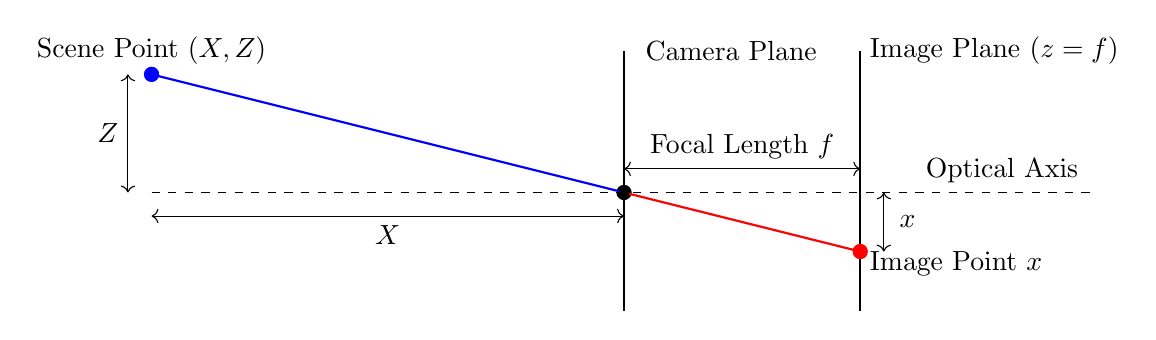
\begin{tikzpicture}[scale=1.5]
  % Draw the image plane
  \draw[thick] (6,0) -- (6,2.2);
  \node[right] at (6,2.2) {Image Plane ($z=f$)};
  % Draw the image plane
  \draw[thick] (4,0) -- (4,2.2);
  \node[right] at (4.1,2.2) {Camera Plane};
  % Draw the optical axis
  \draw[dashed] (0,1) -- (8,1);
  \node[above] at (7.2,1) {Optical Axis};
  % Draw the pinhole (center of projection)
  \filldraw[black] (4,1) circle (0.06);
  % \node[above] at (4.6,0.6) {Pinhole $O$};
  % Draw the scene point (object) on the left
  \filldraw[blue] (0,2) circle (0.06);
  \node[above] at (0,2) {Scene Point $(X,Z)$};
  % Draw projection line from scene point to pinhole
  \draw[blue,thick] (0,2) -- (4,1);
  % Draw projection line from pinhole to image plane (right side)
  \draw[red,thick] (4,1) -- (6,0.5);
  % Draw the projected point on image plane
  \filldraw[red] (6,0.5) circle (0.06);
  \node[right] at (6,0.4) {Image Point $x$};
  % Label distances
  \draw[<->] (0,0.8) -- (4,0.8);
  \node[below] at (2,0.8) {$X$};
  \draw[<->] (-0.2,1) -- (-0.2,2);
  \node[left] at (-0.2,1.5) {$Z$};
  \draw[<->] (6.2,1) -- (6.2,0.5);
  \node[right] at (6.25,0.75) {$x$};
  \draw[<->] (6,1.2) -- (4,1.2);
  \node[above] at (5,1.2) {Focal Length $f$};
  % Draw focal length line
  \draw[dashed] (0,1) -- (4,1);
  \filldraw[black] (4,1) circle (0.04);
\end{tikzpicture}
\end{center}

\vspace{0.3cm}

\noindent from the diagram, we have:

\[
\frac{x}{f} = \frac{X}{Z}
\quad \Rightarrow \quad
x = f \cdot \frac{X}{Z}
\]
Here, $f$ is the focal length of the pinhole camera.


\nt{we use Capital letters for 3D coordinates and lowercase for 2D image coordinates and observe that the \textrm{Z} component is lost.}

\subsection{Pinhole Camera Model (3D)}
Extending to 3D coordinates $(X,Y,Z)$, the projection onto the image plane gives:
\[
x = f \cdot \frac{X}{Z}, \quad
y = f \cdot \frac{Y}{Z}
\]

\noindent This shows how 3D geometry is mapped to 2D via perspective projection.

\subsection{Homogeneous Coordinates}
Homogeneous coordinates are used to express projection as a matrix multiplication:
\[
\begin{bmatrix}x \\ y \\ 1 \end{bmatrix}
= \frac{1}{Z}
\begin{bmatrix}
f & 0 & 0 & 0 \\
0 & f & 0 & 0 \\
0 & 0 & 1 & 0
\end{bmatrix}
\begin{bmatrix} X \\ Y \\ Z \\ 1 \end{bmatrix}
\]

\nt{Homogeneous coordinates are crucial because they unify perspective projection, translation, and rotation into matrix multiplications.}

\subsection{Intrinsic Matrix}
The \textbf{intrinsic parameters} capture camera-specific properties such as focal length and principal point offset:
\[
K =
\begin{bmatrix}
f_x & 0 & c_x \\
0 & f_y & c_y \\
0 & 0 & 1
\end{bmatrix}
\]
where $(f_x,f_y)$ are focal lengths in pixel units and $(c_x,c_y)$ is the principal point.

\subsection{Extrinsic Matrix}
The \textbf{extrinsic parameters} describe the camera’s position and orientation in the world:
\[
M = [R|t]
\]
where $R$ is a $3\times 3$ rotation matrix and $t$ is a $3 \times 1$ translation vector.

\nt{
The rotation matrix $R$ can be defined using an angle $\alpha$ in 2D as:
\[
R(\alpha) = 
\begin{bmatrix}
\cos\alpha & -\sin\alpha \\
\sin\alpha & \cos\alpha
\end{bmatrix}
\]
This matrix rotates a point by $\alpha$ radians in the plane.
% }
% \nt{
In 3D, rotation can be performed about each axis using three matrices:
\[
R_x(\theta) = 
\begin{bmatrix}
1 & 0 & 0 \\
0 & \cos\theta & -\sin\theta \\
0 & \sin\theta & \cos\theta
\end{bmatrix}
% \]
% \[
\quad , \quad
R_y(\phi) = 
\begin{bmatrix}
\cos\phi & 0 & \sin\phi \\
0 & 1 & 0 \\
-\sin\phi & 0 & \cos\phi
\end{bmatrix}
% \]
% \[
\quad , \quad
R_z(\psi) = 
\begin{bmatrix}
\cos\psi & -\sin\psi & 0 \\
\sin\psi & \cos\psi & 0 \\
0 & 0 & 1
\end{bmatrix}
\]
A general 3D rotation can be represented by multiplying these matrices:
\[
R = R_z(\psi) R_y(\phi) R_x(\theta)
\]
where $\theta$, $\phi$, and $\psi$ are rotation angles about the $x$, $y$, and $z$ axes, respectively.

}

\subsection{Projection Matrix}
The complete mapping from 3D world coordinates to 2D image plane is:
\[
s \begin{bmatrix} u \\ v \\ 1 \end{bmatrix}
= K M 
\begin{bmatrix} X \\ Y \\ Z \\ 1 \end{bmatrix}
\]
with scaling factor $s$.  

\clm{Projection Matrix}{}
{The projection matrix $P = K @ M$ completely defines the mapping from world coordinates to image coordinates, which depends on the intrinsic and extrinsic parameters of the camera. (i.e., focal length, principal point, rotation, and translation vectors.)}

% \subsection{Camera Calibration}
\dfn{Camera Calibration}{The process of estimating the intrinsic and extrinsic parameters of a camera from observed images of a known calibration pattern.}
Calibration ensures accurate geometric measurements from images.


\section{Image Representation}

\subsection{Pixel Values}
A digital image is represented as a 2D array of \textbf{pixels (picture elements)}, each encoding intensity (grayscale) or color.


\dfn{Image \& Pixel}{%
An \textbf{image} is a 2D array $$I:\{0,\dots,M-1\}\times\{0,\dots,N-1\}\to\{0,\dots,K-1\}$$
Each element $I[i,j]$ is a \textbf{pixel} with \textbf{intensity} (gray level) in $\{0,\dots,K-1\}$, where, 0 represents black and $K-1$ represents white. For a 8 bit storage, $B = 8$, then maximum intensity can be calculated as $K = 2^B = 2^8 = 256$, $0$ represents black and $255$ represents white. \\

For normalized intensity, use $$I_n[i,j]=\frac{I[i,j]}{(K-1)}\in[0,1]$$.%
}

\subsection{Color Spaces}
Different \textbf{color spaces} represent pixel values differently:
\begin{itemize}
    \item RGB: additive primary colors.
    \item HSV: hue, saturation, value (closer to human perception).
    \item YCbCr: luminance and chrominance separation. (where Y is intensity)
\end{itemize}



\subsection{Feature Extraction and Descriptors}
\textbf{Features} capture essential information in images such as edges, corners, or textures.  
\textbf{Descriptors} encode features into numerical representations (e.g., SIFT, HOG) for matching and recognition.

\subsection{Sampling and Quantization}
The ideal irradiance signal is sampled on a discrete grid and quantized to a finite set of gray levels.
\begin{itemize}
    \item \textbf{Sampling:} Selecting discrete spatial points to represent an image.\\
    choose integer pixel sites $(i,j)$; the image becomes $I[i,j]$ on an $M\times N$ grid.
    \item \textbf{Quantization:} Mapping continuous intensity values into discrete levels \\
    map real intensities to $\{0,1,\dots,K-1\}$, e.g., $K=256$ for 8-bit grayscale.
\end{itemize}

\noindent \textbf{Binary images:} special case $K=2$ with intensities $\{0,1\}$ (or $\{0,255\}$ in 8-bit storage).



\nt{Undersampling causes aliasing; inadequate quantization leads to loss of detail.}

\subsection{Image Formats}
Typical resolutions include $256\times 256$, $512\times 512$, \textbf{1920x1080}, etc.%
As we can calculate the number of Bytes required to store these images, we find:

\begin{itemize}
    \item For $256\times 256$ images: $256 \times 256 \times 1 = 65,536$ Bytes (assuming 8-bit grayscale).
    \item For $512\times 512$ images: $512 \times 512 \times 1 = 262,144$ Bytes (assuming 8-bit grayscale).
    \item For $1920\times 1080$ images: $1920 \times 1080 \times 3 = 6,220,800$ Bytes (assuming 24-bit RGB).
\end{itemize}

which is nearly 6.3 MB for a full HD image (1920x1080 3-channel RGB image). 
Hence, image storage can be quite substantial, necessitating efficient compression techniques. \\

Few common \textbf{Formats} include:
\begin{itemize}
    \item JPEG: lossy compressed format. \\
    The most common for photographs to save space, as the human eye is less sensitive to high-frequency details. The compression is achieved by discarding some image data, but the benefit is a significantly reduced file size. (e.g. the full HD image (1920x1080) can be compressed from {\bf 6.3 MB} to around less than a {\bf 1 MB})
    \item PNG: lossless compression, supports transparency.
    \item BMP: uncompressed raster format.
    \item TIFF: flexible format supporting various compressions.
    \item GIF: supports animation and transparency (limited color palette).
    \item WEBP: modern format providing lossy and lossless compression.
    \item HEIF: high efficiency image format, supports advanced features.
    \item AVIF: image format based on AV1 compression, offering high quality at smaller file sizes.
    \item EXR: high dynamic range (HDR) image format, supports wide color gamuts and high bit depths.
    \item DNG: raw image format for digital photography, preserves original sensor data.
    \item PPM: portable pixmap format, simple uncompressed color image format.
\end{itemize}

\subsection{Binary Images and Thresholding}

\dfn{Binary Image}{
A \textbf{binary image} is an image that consists of only two colors, typically black and white. Each pixel in a binary image is represented by a single bit, where 0 represents black and 1 represents white.
}


\noindent The simplest method to obtain binary images is \textbf{thresholding}:
\[
B(x,y) = \begin{cases}
1 & I(x,y) \geq T \\
0 & I(x,y) < T
\end{cases}
\]
where $T$ is the threshold.

\subsection{Gray Level Histograms}
The histogram of grayscale values is a fundamental tool to analyze and design thresholding algorithms.

\clm{Histogram-based Thresholding}{}
{If the histogram shows two well-separated peaks, the optimal threshold lies near the valley between them.}



%==========================
\section{Histogram of an Image}
%==========================

\dfn{Gray-Level Histogram}{
A \textbf{gray-level histogram} is a representation of the distribution of pixel intensities in a grayscale image. It counts the number of pixels for each intensity level, providing insights into the image's contrast and brightness.
}
\paragraph{Mathematical Formulation}

Let a grayscale image be
$$I:\{0,\dots,M\!-\!1\}\times\{0,\dots,N\!-\!1\}\to\{0,\dots,K\!-\!1\}$$. 
The \emph{histogram} counts occurrences at each gray level, given as a function as 
$$H:\{0,\dots,K\!-\!1\}\to\{0,\dots,MN\}$$

such that 
$$ H(k) = \text{no of occurrences of gray level } k$$ 

where $k \in \{0,\dots,K-1\}$

\[
H(k) \;=\; \#\{(i,j): I[i,j]=k\} \qquad k=0,\dots,K-1
\]

also, 
\[
\sum_{k=0}^{K-1} H(k)=MN.
\]

\noindent The \emph{normalized histogram} (PMF) is $$p(k)=\tfrac{H(k)}{MN}$$

and $$\sum_k p(k)=1$$


\ex{Interpreting Histogram Shapes}{
Given an image whose histogram exhibits a tall peak near intensity $40$ (dark shades), and another smaller, broad peak near $200$ (bright shades), we deduce the image features a dark background with a bright foreground—ideal for segmentation via thresholding.

\begin{itemize}
\item \textbf{Dark image:} $p(k)$ concentrated near $k\approx 0$.
\item \textbf{Bright image:} $p(k)$ concentrated near $k\approx K\!-\!1$.
\item \textbf{Bimodal image:} two peaks (e.g., dark foreground on bright background) $\Rightarrow$ suitable for a \emph{single} global threshold.
\end{itemize}

\begin{center}
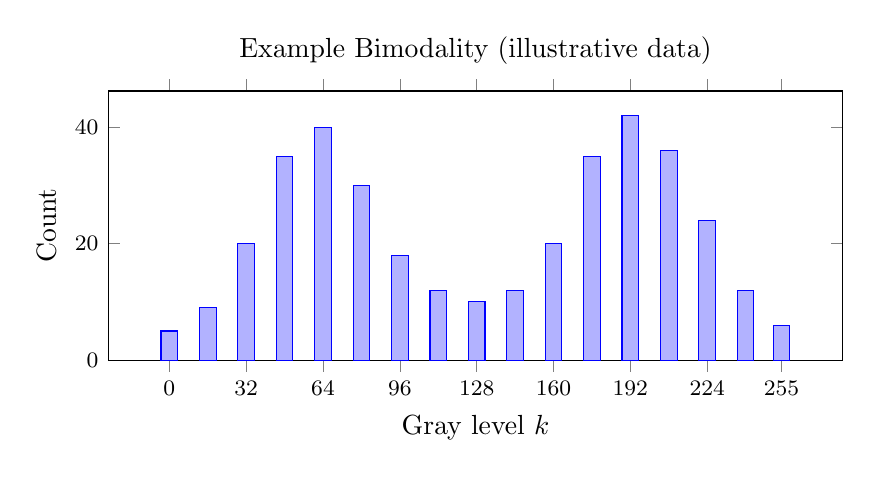
\begin{tikzpicture}
\begin{axis}[
  ybar, bar width=6pt, width=0.9\linewidth, height=5cm,
  ymin=0, ylabel={Count}, xlabel={Gray level $k$},
  xtick={0,32,64,96,128,160,192,224,255},
  xticklabel style={font=\footnotesize}, yticklabel style={font=\footnotesize},
  title={Example Bimodality (illustrative data)}
]
\addplot coordinates {(0,5) (16,9) (32,20) (48,35) (64,40) (80,30) (96,18) (112,12)
(128,10) (144,12) (160,20) (176,35) (192,42) (208,36) (224,24) (240,12) (255,6)};
\end{axis}
\end{tikzpicture}
\end{center}
}

% Gray level image histograms are foundational tools in digital image processing, providing a statistical representation of the distribution of pixel intensities in an image. The histogram constitutes an array or plot where the $x$-axis denotes possible gray levels (e.g., $0$ to $255$ for 8-bit images), and the $y$-axis gives the count or probability of each gray level's appearance within the image.

\nt{Understanding the histogram profile assists in identifying whether an image is underexposed, overexposed, well-contrasted, or subject to other illumination artifacts.}


\paragraph{Types of Histograms and Their Interpretation}
Different histogram profiles relate directly to the visual impression and underlying properties of an image:
\begin{itemize}
    \item \textbf{Bright Images:} Most pixel values clustered towards the higher end of the gray level range.
    \item \textbf{Dark Images:} Values crowded in the lower end, leading to overall darker visual output.
    \item \textbf{Dual Peak Model:} Exhibits two pronounced peaks, often corresponding to distinct foreground and background regions; common in images fit for binarization.
    \item \textbf{Flat Histogram:} Pixels uniformly distributed across gray levels—rare in natural images, may occur in images heavily corrupted with noise.
    \item \textbf{Equal Histograms:} Result from histogram equalization operations to improve contrast.
\end{itemize}

\ex{Histogram Interpretation}{
\begin{itemize}
    \item A \textbf{bright image} shows histogram concentrated on high intensity values.
    \begin{center}
      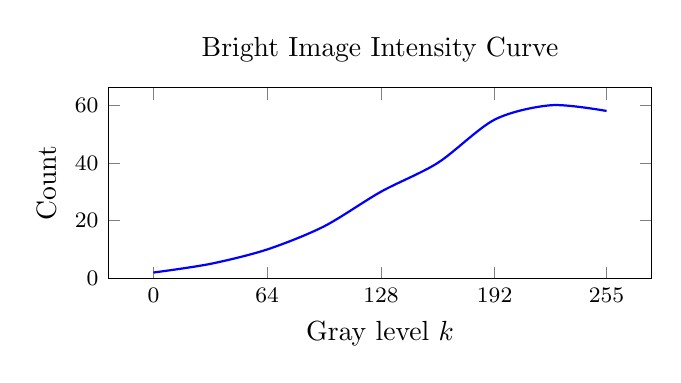
\begin{tikzpicture}
      \begin{axis}[
        width=0.7\linewidth, height=4cm,
        ymin=0, ylabel={Count}, xlabel={Gray level $k$},
        xtick={0,64,128,192,255},
        xticklabel style={font=\footnotesize}, yticklabel style={font=\footnotesize},
        title={Bright Image Intensity Curve}
      ]
      % Smooth curve through the points
      \addplot[
        smooth, thick, blue
      ] coordinates {
        (0,2) (32,5) (64,10) (96,18) (128,30) (160,40) (192,55) (224,60) (255,58)
      };
      \end{axis}
      \end{tikzpicture}
      \\
      \emph{Intensity profile of a bright image: curve shifted towards high gray levels}
    \end{center}
    \item A \textbf{dark image} shows histogram concentrated on low values.
    \begin{center}
      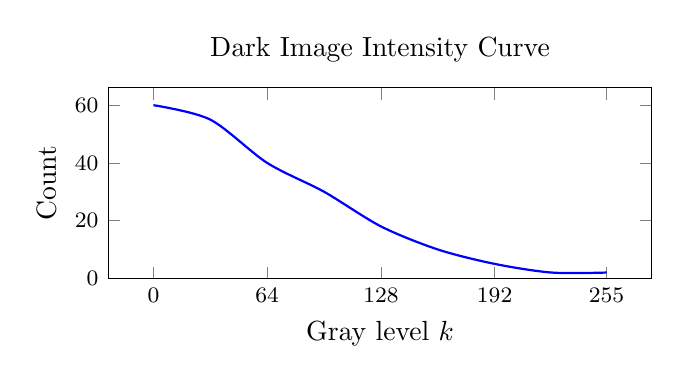
\begin{tikzpicture}
      \begin{axis}[
        width=0.7\linewidth, height=4cm,
        ymin=0, ylabel={Count}, xlabel={Gray level $k$},
        xtick={0,64,128,192,255},
        xticklabel style={font=\footnotesize}, yticklabel style={font=\footnotesize},
        title={Dark Image Intensity Curve}
      ]
      % Smooth curve through the points
      \addplot[
        smooth, thick, blue
      ] coordinates {
        (0,60) (32,55) (64,40) (96,30) (128,18) (160,10) (192,5) (224,2) (255,2)
      };
      \end{axis}
      \end{tikzpicture}
      \\
      \emph{Intensity profile of a dark image: curve shifted towards low gray levels}
    \end{center}
    \item A \textbf{dual-peak image} indicates presence of both dark (background) and bright (foreground) regions.
    \begin{center}
      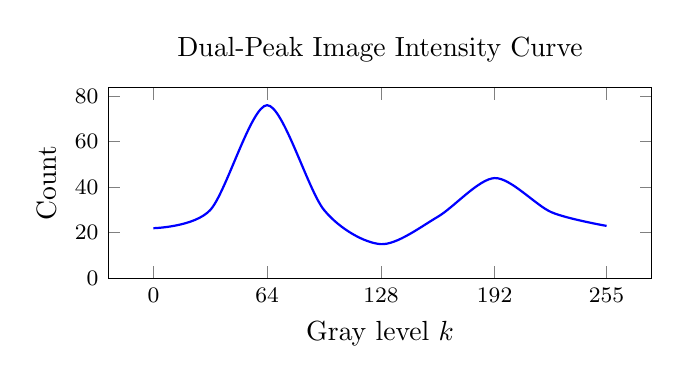
\begin{tikzpicture}
      \begin{axis}[
        width=0.7\linewidth, height=4cm,
        ymin=0, ylabel={Count}, xlabel={Gray level $k$},
        xtick={0,64,128,192,255},
        xticklabel style={font=\footnotesize}, yticklabel style={font=\footnotesize},
        title={Dual-Peak Image Intensity Curve}
      ]
      % Smooth curve through the points
      \addplot[
        smooth, thick, blue
      ] coordinates {
        (0,22) (32,30) (64,76) (96,30) (128,15) (160,27) (192,44) (224,29) (255,23)
      };
      \end{axis}
      \end{tikzpicture}
      \\
      \emph{Intensity profile of a dual-peak image: two distinct peaks at low and high gray levels}
    \end{center}

    \item A \textbf{flat histogram} corresponds to uniformly distributed intensities.
    \begin{center}
      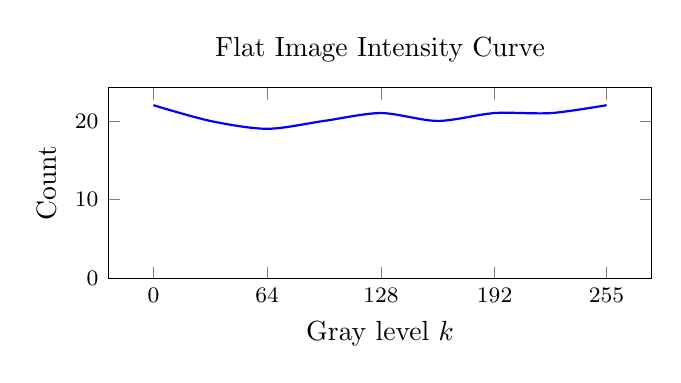
\begin{tikzpicture}
      \begin{axis}[
        width=0.7\linewidth, height=4cm,
        ymin=0, ylabel={Count}, xlabel={Gray level $k$},
        xtick={0,64,128,192,255},
        xticklabel style={font=\footnotesize}, yticklabel style={font=\footnotesize},
        title={Flat Image Intensity Curve}
      ]
      % Smooth curve through the points
      \addplot[
        smooth, thick, blue
      ] coordinates {
        (0,22) (32,20) (64,19) (96,20) (128,21) (160,20) (192,21) (224,21) (255,22)
      };
      \end{axis}
      \end{tikzpicture}
      \\
      \emph{Intensity profile of a flat image: uniform distribution across all gray levels}
    \end{center}

\end{itemize}

\textbf{At a Glance:}

\begin{center}
\renewcommand{\arraystretch}{1.2}
\begin{tabular}{@{}p{3.2cm}p{4.8cm}p{4.8cm}@{}}
\toprule
\textbf{Histogram Type} & \textbf{Typical Scene} & \textbf{Segmentation Implication} \\
\midrule
Dark-skewed & Low-light or dark objects & Threshold near lower gray levels \\
Bright-skewed & Bright background/lighting & Threshold near higher gray levels \\
Bimodal & Foreground vs.\ background & Global threshold often effective \\
Flat/noisy & Low contrast/high noise & Consider contrast stretch or adaptive threshold \\
\bottomrule
\end{tabular}
\end{center}


}


\section{Otsu's Binarization}

Otsu’s thresholding is a non-parametric, unsupervised method for automatic image binarization. It determines the optimal threshold to separate foreground and background by maximizing inter-class variance.

\subsection{Probability and Statistical Prerequisites}

\paragraph{Basic Probability Concepts}
Consider an image histogram with $L$ gray levels ($0, 1, ..., L-1$). Let $p_k$ denote the normalized probability for gray level $k$:
$$
p_k = \frac{n_k}{N}
$$
where $n_k$ is the number of pixels with gray level $k$, and $N$ is the total pixel count.

\subsubsection{Class Probabilities, Means, and Variances}
For a given threshold $T$:

\noindent \textbf{Class Probability}
\begin{itemize}
\item Probability that the pixel belongs to class 0 (background)
\[
\omega_0(T) = \sum_{k=0}^T p _k \quad\text{(Probability of class 0 - background - black pixels)}
\]
\item Probability that the pixel belongs to class 1 (foreground)
\[\omega_1(T) = \sum_{k=T+1}^{L-1} p_k \quad\text{(Probability of class 1 - foreground - white pixels)} 
\]
\end{itemize}

\noindent \textbf{Class Means} 
\begin{itemize}
  

\item  Probability that the pixel takes values k given that it belongs to class 0
\begin{align*}
\mu_0(T) &= \sum_{k=0}^T k \cdot p(k | C_0)  \quad\text{(Mean of class 0)} \\
\text{where} \quad p(k | C_0) &= \frac{p(k, C_0)}{p(C_0)} = \frac{p_k p(C_0 | k)}{p(C_0)} \\
\text{for} k \in \{ 0\dots T \} \quad p(k | C_0) &= \frac{p_k}{\omega_0(T)} \\
\mu_0(T) &=\frac{1}{\omega_0(T)} \sum_{k=0}^T k p_k \\
\text{also, for} k \in \{ T+1 \dots L-1 \} \quad p(k | C_0) &= 0\\ 
\mu_0(T) &=\frac{1}{\omega_0(T)} \sum_{k=0}^{L-1} k p_k
\end{align*}
\item Probability that the pixel takes values k given that it belongs to class 1
\begin{align*}
\mu_1(T) &= \sum_{k=T+1}^{L-1} k \cdot p(k | C_1)  \quad\text{(Mean of class 1)} \\
\text{where} \quad p(k | C_1) &= \frac{p(k, C_1)}{p(C_1)} = \frac{p_k p(C_1 | k)}{p(C_1)} \\
\text{for} k \in \{ T+1 \dots L-1 \} \quad p(k | C_1) &= \frac{p_k}{\omega_1(T)} \\
\mu_1(T) &=\frac{1}{\omega_1(T)} \sum_{k=T+1}^{L-1} k p_k \\
\text{also, for} k \in \{ 0 \dots T \} \quad p(k | C_1) &= 0\\
\mu_1(T) &=\frac{1}{\omega_1(T)} \sum_{k=0}^{L-1} k p_k
\end{align*}

\item Overall Image Mean
\begin{align*}
\mu_T &= \sum_{k=0}^{L-1} k p_k \\
&= \sum_{k=0}^{T} k p_k + \sum_{k=T+1}^{L-1} k p_k\\ 
&= \mu_0(T) \omega_0(T) + \mu_1(T) \omega_1(T)
\end{align*}
\end{itemize}

\noindent \textbf{Class Variances}\\
\begin{itemize}
\item Variance of class 0
\begin{align*}
\sigma_0^2(T) &= \sum_{k=0}^{T} (k - \mu_0(T))^2 p(k | C_0)\\
&= \sum_{k=0}^{T} (k - \mu_0(T))^2 \frac{p_k}{\omega_0(T)}
\end{align*}

\item Variance of class 1
\begin{align*}
\sigma_1^2(T) &= \sum_{k=T+1}^{L-1} (k - \mu_1(T))^2 p(k | C_1)\\
&= \sum_{k=T+1}^{L-1} (k - \mu_1(T))^2 \frac{p_k}{\omega_1(T)}
\end{align*}

\item Total Image Variance
\begin{align*}
  \sigma^2 (T) &= \sum_{k=0}^{L-1} (k - \mu_T)^2 p_k \\
  &= \sum_{k=0}^{T} (k - \mu_T)^2 p_k + \sum_{k=T+1}^{L-1} (k - \mu_T)^2 p_k \\
  &= \sigma_0^2(T) + \sigma_1^2(T) + \omega_0(T)[\mu_0(T) - \mu_T]^2 + \omega_1(T)[\mu_1(T) - \mu_T]^2
\end{align*}
\end{itemize}

\dfn{Within Class Variance $\sigma_w^2(T)$}{
  The variance of pixel intensities within class is given by:
  \begin{align*}
  \sigma_w^2(T) &= \omega_0(T) \sigma_0^2(T) + \omega_1(T) \sigma_1^2(T)
  \end{align*}

  Also known as intra-class variance, $\sigma_w^2(T)$ measures the compactness of pixel intensities within each class. \textbf{maximizing} $\sigma_w^2(T)$ leads to better class separability.
}

\dfn{Between Class Variance $\sigma_b^2(T)$}{
  The variance of pixel intensities between class is given by:
  \begin{align*}
  \sigma_b^2(T) &= \sigma^2 - \sigma_w^2(T) \\
  &= \sigma^2 - \left( \omega_0(T) \sigma_0^2(T) + \omega_1(T) \sigma_1^2(T) \right)\\
  &= \omega_0(T) \omega_1(T) \left[ \mu_0(T) - \mu_1(T) \right]^2
  \end{align*}

  Also known as inter-class variance, $\sigma_b^2(T)$ measures the separability of pixel intensities between classes. \textbf{minimizing} $\sigma_w^2(T)$ leads to better class compactness.
}

\subsection{Otsu’s Binarization: Statement and Algorithm}

\dfn{Otsu’s Binarization}{The process of determining the threshold $T^*$ that maximizes the inter-class variance between foreground and background, thus optimally segmenting a bimodal histogram image.}

\begin{center}
\begin{tikzpicture}[scale=1.2]
    % Axis
    \draw[->] (0,0) -- (5,0) node[right] {Intensity};
    \draw[->] (0,0) -- (0,3) node[above] {Histogram};
    % Bimodal histogram
    \draw[domain=0.3:2.3,smooth,variable=\x,blue,thick] plot (\x,{2*exp(-2*(\x-1)^2)});
    \draw[domain=2.7:4.7,smooth,variable=\x,red,thick] plot (\x,{2*exp(-2*(\x-4)^2)});
    % Threshold line at T
    \draw[dashed] (2.5,0) -- (2.5,2) node[above] {$T^*$};
\end{tikzpicture}

\textit{A typical bimodal histogram: $T^*$ chosen to best separate two peaks.}
\end{center}

\paragraph{Optimization Criteria}

Otsu’s method selects a threshold $T^*$ to partition the image pixels into two classes (often foreground and background) so that the variance between these classes (\textbf{inter-class variance}) is maximized, or equivalently, the variance within each class (\textbf{intra-class variance}) is minimized. These criteria are mathematically dual—maximizing $\sigma_b^2(T)$ is identical to minimizing $\sigma_w^2(T)$ since their sum is the total variance $\sigma^2$.

\clm{Equivalence of Maximization and Minimization Criteria}{}{
Maximizing the between-class variance $\sigma_b^2(T)$ is equivalent to minimizing within-class variance $\sigma_w^2(T)$, as
\[
\arg\max_T \sigma_b^2(T) = \arg\min_T \sigma_w^2(T)
\]
since $\sigma^2$ is fixed for a given image histogram.
}
\nt{In practice, Otsu's method typically maximizes $\sigma_b^2(T)$, but formulations based on minimizing $\sigma_w^2(T)$ yield the same optimal threshold $T^*$.}

\subsection{Method 1: Maximization of Inter-Class Variance}

Threshold $T^*$ is selected to maximize the between-class variance $\sigma_b^2(T)$.
$$
  T^* = \arg\max_T \sigma_b^2(T) = \arg\max_T \left[ \omega_0(T) \omega_1(T) \left( \mu_0(T) - \mu_1(T) \right)^2 \right]
$$

\noindent The algorithm for Otsu's binarization by maximizing $\sigma_b^2(T)$ is as follows:

\begin{enumerate}
    \item Compute the histogram and probabilities $p_i = n_i/N$ for each gray level $i$.
    \item For each possible threshold $T$ (from gray level $1$ to $L-2$):
    \begin{itemize}
        \item Calculate class weights (probabilities): $\omega_0(T)$ and $\omega_1(T)$.
        \item Calculate class means: $\mu_0(T)$ and $\mu_1(T)$.
        \item Compute between-class variance:
            \[
            \sigma_b^2(T) = \omega_0(T)\,\omega_1(T)\left[\mu_0(T) - \mu_1(T)\right]^2
            \]
    \end{itemize}
    \item Find the threshold $T^*$ that maximizes $\sigma_b^2(T)$.
\end{enumerate}

\ex{Numerical Example}{
Suppose an image has normalized histogram values:
$
p_0 = 0.4, \quad p_1 = 0.2, \quad p_2 = 0.2, \quad p_3 = 0.2
$
Try threshold $T = 1$:
\begin{align*}
\omega_0(1) &= p_0 + p_1 = 0.6\\
\omega_1(1) &= 0.4\\
\mu_0(1) &= \frac{0 \cdot 0.4 + 1 \cdot 0.2}{0.6} = 0.333\\
\mu_1(1) &= \frac{2 \cdot 0.2 + 3 \cdot 0.2}{0.4} = 2.5
\end{align*}
Now,
\[
\sigma_b^2(1) = 0.6 \times 0.4 \times (0.333 - 2.5)^2 \approx 0.6 \times 0.4 \times 4.694 \approx 1.126
\]
similarly for $T=2$:
\begin{align*}
\omega_0(2) &= p_0 + p_1 +p_2 = 0.8\\
\omega_1(2) &= 0.2\\
\mu_0(2) &= \frac{0 \cdot 0.4 + 1 \cdot 0.2 + 2 \cdot 0.2}{0.8} = 0.75\\
\mu_1(2) &= \frac{3 \cdot 0.2}{0.2} = 3
\end{align*}
Now,
\[
\sigma_b^2(2) = 0.8 \times 0.2 \times (0.75 - 3)^2 \approx 0.8 \times 0.2 \times 5.0625 \approx 0.81
\]

\begin{center}
\renewcommand{\arraystretch}{1.3}
\begin{tabular}{c|c|c|c|c|c}
\toprule
$T$ & $\omega_0(T)$ & $\omega_1(T)$ & $\mu_0(T)$ & $\mu_1(T)$ & $\sigma_b^2(T)$ \\
\midrule
1 & 0.6 & 0.4 & 0.3333 & 2.5 & \textbf{1.1267} \\
2 & 0.8 & 0.2 & 0.75 & 3 & 0.81 \\
\bottomrule
\end{tabular}
\end{center}

\[
\boxed{\text{Maximum } \sigma_b^2 \text{ occurs at } T=1, \quad
\sigma_b^2(1)\approx \mathbf{1.1267}.}
\]

}

\subsection{Method 2: Minimization of Within-Class Variance}

Threshold $T^*$ is selected to minimize the within-class variance $\sigma_w^2(T)$.
$$
  T^* = \arg\min_T \sigma_w^2(T) = \arg\min_T \left[ \omega_0(T) \sigma_0^2(T) + \omega_1(T) \sigma_1^2(T) \right]
$$

\noindent This approach explicitly minimizes intra-class variance $\sigma_w^2(T)$.

\begin{enumerate}
    \item For each threshold $T$, calculate:
    \begin{align*}
        \sigma_w^2(T) = \omega_0(T) \sigma_0^2(T) + \omega_1(T) \sigma_1^2(T)
    \end{align*}
    where $\sigma_k^2(T)$ are variances for classes $k=0,1$, based on histogram statistics within each class.
    \item Find $T^*$ that minimizes $\sigma_w^2(T)$.
\end{enumerate}

\clm{Proof of Equivalence}{}{
Since $\sigma^2 = \sigma_w^2(T) + \sigma_b^2(T)$ for all $T$, maximizing $\sigma_b^2(T)$ is the same as minimizing $\sigma_w^2(T)$.
}
\nt{For both criteria, iterate over possible $T$ to find the optimal value. Both algorithms yield identical results provided all statistics are computed correctly.}

\subsection{Algorithm Summary: Otsu’s Binarization (most used)}

\begin{enumerate}
    \item Compute image histogram.
    \item For each threshold $T$:
    \begin{itemize}
        \item Partition pixels into two classes.
        \item Compute $\omega_k(T)$, $\mu_k(T)$, $\sigma_k^2(T)$ as needed.
        \item Compute either $\sigma_b^2(T)$ or $\sigma_w^2(T)$.
    \end{itemize}
    \item Determine $T^*$ by maximizing $\sigma_b^2(T)$ or minimizing $\sigma_w^2(T)$.
    \item Binarize the image: pixels $\leq T^*$ are assigned to class 0; others to class 1.
\end{enumerate}

\nt{Otsu’s method is most effective for bimodal histograms, but may be suboptimal for multi-modal or unimodal histograms. Variations and generalizations (multi-level, local thresholding) exist for more complex cases.}

% !TEX root=./../maha-dip-notes.tex
\chapter{Gray Scale Image Processing}

\section{Point Operations}

Point operations are image transformations where each output pixel is computed solely from its corresponding input pixel, without regard for neighboring values.

\dfn{Point Operation}{A transformation applied to each pixel individually, $J(x,y) = T[I(x, y)]$, where $I(x, y)$ is the input image and $T$ is a point-wise mapping function.}

These operations can be linear or non-linear, and are different from local operators/spatial filters (i.e., those that consider neighboring pixels such as ERODE, DILATE, etc.).

No explicit neighborhood information is used in point operations, and no explicit modifications based on spatial context. however, they can still be influenced by global image properties (e.g., overall brightness, contrast).



\subsection{Image Offset (Brightness Adjustment)}
The simplest point operation is the offset, where a constant value $c$ is added to all pixel intensities:
$$
J(x, y) = I(x, y) + c
$$
This increases (or decreases) the brightness of the image uniformly.
\begin{itemize}
    \item If $c > 0$, the image becomes brighter.
    \item If $c < 0$, the image becomes darker.
\end{itemize}

\ex{Image Offset Application}{
    Suppose $I_1,I_2,\dots, I_N$ are $N$ images of the same scene taken under different lighting conditions (different exposures). If we wish to equalise all their average intensities to $\frac{K}{2}$ (where K is number of intensity levels), a point operation can be used to normalize brightness across these images by applying an offset to each image:
    $$J_i(x, y) = I_i(x, y) + c_i$$
    where $c_i$ is the offset computed as:
    $$c_i = \frac{K}{2} - \text{mean}(I_i)$$
}

\subsection{Image Scaling (Contrast Adjustment)}
Image scaling multiplies all pixel intensities by a constant factor $a$:
$$
J(x, y) = a \cdot I(x, y)
$$
A scaling factor $a > 1$ increases contrast, while $0 < a < 1$ darkens the image.


\subsection{Offset and Scaling}
Combining offset and scaling operations allows for more flexible image adjustments. The combined operation can be expressed as:
$$
J(x, y) = a \cdot I(x, y) + c
$$
Where $a$ is the scaling factor and $c$ is the offset. This allows for both contrast adjustment (via scaling) and brightness adjustment (via offset) in a single operation.

\ex{Negative Image}{
    The negative of an image is obtained by inverting the pixel values by choosing :
    \begin{itemize}
        \item image offset  $c = K - 1$, Where $K$ is the number of intensity levels.
        \item image scaling $a = -1$
    \end{itemize}
    Thus,
    $$
    J(x, y) = K - 1 - I(x, y)
    $$
    This operation effectively reverses the brightness levels, making dark areas light and vice versa.
}

\ex{Full Scale Contrast stretch}{
    Let A \& B be the minimum and maximum intensity values in the image respectively. We wish to stretch the contrast to full scale $[0, K-1]$. This can be achieved from $aA + c = 0$ and $aB + c = K - 1$, we can solve for $a$ and $c$, we get:
    \begin{itemize}
        \item image scaling $a = \frac{K-1}{B-A}$
        \item image offset  $c = -\frac{K-1}{B-A} \cdot A$
    \end{itemize}
    Thus,
    \begin{align*}
    J(x, y) &= \frac{K-1}{B-A} \cdot I(x, y) - \frac{K-1}{B-A} \cdot A\\
    &= \frac{K-1}{B-A} \cdot (I(x, y) - A)
    \end{align*}
    This allows us to stretch the pixel values to cover the full range of intensities, hence enhances the overall contrast of the image.
}

\subsection{Non-linear Point Operations}
Non-linear point operations are techniques that apply non-linear transformations to the pixel values of an image. These operations can enhance certain features or suppress others, depending on the specific transformation applied.

\paragraph{Common Examples}
\begin{itemize}
    
    \item \textbf{Gamma Correction:}
        $$
        J(x, y) = c \cdot I(x, y)^\gamma \qquad \gamma > 0
        $$
        Where $c$ is a scaling factor and $\gamma$ is the gamma value.
        \begin{itemize}
            \item $0 < \gamma < 1$ : Enhances dark regions (gamma correction).
            \item $\gamma > 1$ : Enhances bright regions (inverse gamma correction).
        \end{itemize}

        \begin{center}
        \begin{tikzpicture}
            \draw[->] (0,0) -- (5,0) node[right] {Input Intensity};
            \draw[->] (0,0) -- (0,5) node[above] {Output};
            \draw[domain=0:5,smooth,variable=\x,blue,thick] plot (\x,{pow(\x/5,0.5)*5});
            \draw[domain=0:5,smooth,variable=\x,red,dashed] plot (\x,{pow(\x/5,2)*5});
            % Two gamma curves: gamma=0.5 (blue, boost), gamma=2 (red, dampen)
        \end{tikzpicture}
        \\
        \emph{Gamma Correction ( Blue : $\gamma = 0.5 \rightarrow I^{\frac{1}{2}}$  , Red : $\gamma = 2 \rightarrow I^{2}$ )}
        \end{center}

    \item \textbf{Sigmoid Correction:}
        $$
        J(x, y) = \frac{K}{1 + \exp(-\beta [I(x, y) - \alpha])}
        $$
        Where $K$ is maximal intensity, $\alpha$ the mid-point, and $\beta$ the slope. Useful for contrast enhancement around a chosen intensity.

        \begin{center}
        \begin{tikzpicture}
            \draw[->] (0,0) -- (5,0) node[right] {Input Intensity};
            \draw[->] (0,0) -- (0,5) node[above] {Output};
            \draw[domain=0:5,smooth,variable=\x,blue,thick] plot (\x,{5/(1 + exp(-9*(\x/5-0.5)))});
            % Sigmoid curve: midpoint at 0.5, slope=9
        \end{tikzpicture}
        \\
        \emph{Sigmoid Correction Curve}
        \end{center}


    \item \textbf{Other Non-linear Operations:}
        \begin{itemize}
            \item \emph{Logarithmic Correction:} $g(x, y) = c \cdot \log(1 + f(x, y))$
            \item \emph{Exponential Correction:} $g(x, y) = a \cdot \exp(f(x, y)/b)$
            \item \emph{Piece-wise Linear Transformations:} used for specific intensity mapping (e.g., contrast stretching).
        \end{itemize}
\end{itemize}



\nt{Non-linear point operations are often employed to address unique characteristics of image acquisition (camera response, display systems) or to prepare images for further processing steps like thresholding or segmentation.}



\section{Histogram Equalization}

Histogram equalization is a method to adjust image intensities to enhance contrast. The histogram of an image is "flattened" (equalized), redistributing pixel values as uniformly as possible over the intensity range.

\dfn{Histogram Equalization}{A point-wise image transformation that remaps the intensity distribution so that the output histogram is (approximately) uniform. This increases the dynamic range and enhances global contrast.}

\noindent Given a gray scale image with intensities $r$ in $[0, K-1]$ and histogram $h(r)$, histogram equalization computes a transformation $HE$ as the cumulative distribution function (CDF):
$$
HE(r) = \sum_{k=0}^{r} \frac{h(k)}{MN}
$$
where $MN$ is the total number of pixels.

\dfn{Histogram Equalization Transformation}{
The transformation $s = HE(r)$ maps each input intensity $r$ to an output intensity $s$ so that $s$ is approximately uniformly distributed over $[0, K-1]$.
}

% % !TEX root=./../maha-dip-notes.tex
\chapter{Frequency Domain Processing}
\label{lec_03}
% !TEX root=./../maha-dip-notes.tex
\section{Prerequisites for Fourier Transforms}
\label{lec_03_sec_01}

% % !TEX root=./../maha-dip-notes.tex
\section{}
\label{lec_03_sec_02}
% % !TEX root=./../maha-dip-notes.tex
\section{}
\label{lec_03_sec_03}
% % !TEX root=./../maha-dip-notes.tex
\section{}
\label{lec_03_sec_04}
% % !TEX root=./../maha-dip-notes.tex
\section{}
\label{lec_03_sec_05}


% % !TEX root=./../maha-dip-notes.tex
\chapter{Image Restoration}

\section{Introduction}

% % !TEX root=./../maha-dip-notes.tex
\chapter{Image Features}

\section{Introduction}



\bibliographystyle{siam}
\bibliography{refs.bib}

\end{document}
